\chapter{Evaluation}
\label{chapter:chapter5}

\section{Evaluation System}
\label{sec:testing-system}

For evaluating the system we used a few machines to test if the system components are able to communicate from independent machines. We used one machine for each type of component: one for the WordPress server, one for the Workload Generator, and a third one for the Controller component. Each of them had an AMD Phenom 9600B Quad-Core processor with 2293 MHz CPU and 2GB of memory. For the last part of the tests we used two machines with Intel Core 2Duo Processor with 2.00GHz CPU and 2GB of memory. On one machine was placed the WordPress server, and on the second one the Workload Generator and the Controller.

\section{Evaluation Results}
\label{sub-sec:test-results}

During system evaluation we varied a number of inputs:
\begin{itemize}
 \item number of users
 \item read-only ratio
 \item simulation length
\end{itemize}

We ran tests with a constant number of 50 users, so this is why the resulting graphs \labelindexref{Figure}{figure:graph0}, \labelindexref{Figure}{figure:graph1} and \labelindexref{Figure}{figure:graph2} have a constant response time, situated within a range. We then ran the benchmark with an increasing number of users, from 50 users to 80 and the response time increase can be observed in \labelindexref{Figure}{figure:graph3}. We also ran tests with a slightly larger number of users, 100 and 300, and the results are depicted in \labelindexref{Figure}{figure:graph4} and \labelindexref{Figure}{figure:graph5}.

Afterwards we varied the read-only ratio from value 0.4 in \labelindexref{Figure}{figure:graph0}, \labelindexref{Figure}{figure:graph4} and \labelindexref{Figure}{figure:graph5}, to value 0  in \labelindexref{Figure}{figure:graph1}, and value 1 in \labelindexref{Figure}{figure:graph2}. The simulation length was 15-20 minutes, excluding the initialization step. We observed that user creation step take a quite large amount of time, so this is why the simulations with larger number of users have a bigger relative time (placed on OX axis).

The evaluation process unveiled a few issues, the biggest one being the long login time and user creation time. This increased the overall response time dramatically, and the spikes present in the graphs are caused by these long delays. 

\begin{figure}[ht]
  \centering %trim=l b r t
  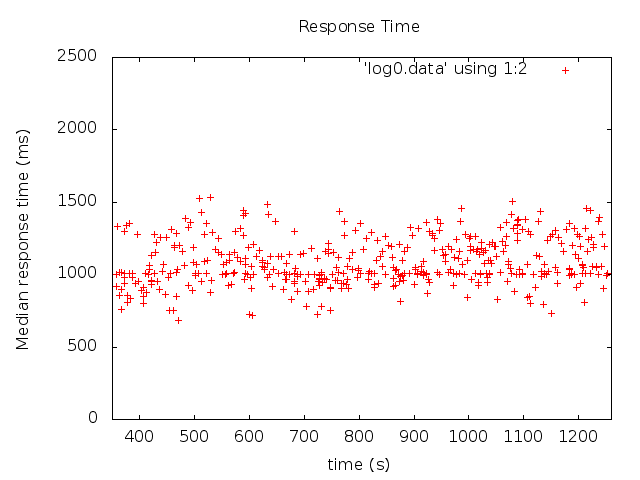
\includegraphics[scale=0.5]{src/img/out0.png}
  \caption{A benchmark evaluation with 0.4 Read-only ratio}
\label{figure:graph0}
\end{figure}

\begin{figure}[ht]
  \centering %trim=l b r t
  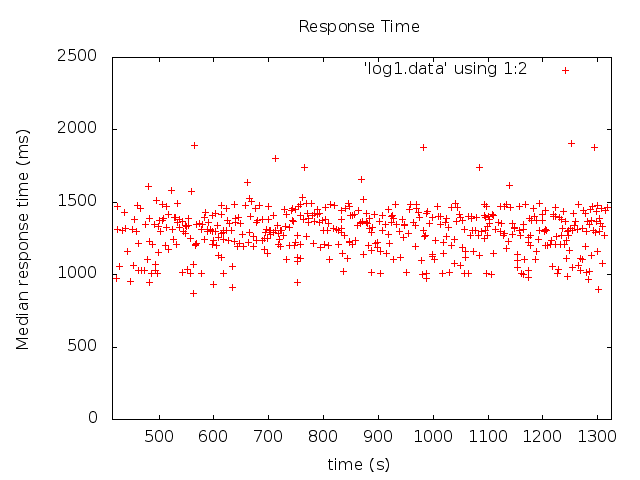
\includegraphics[scale=0.5]{src/img/out1.png}
  \caption{A benchmark evaluation with 0.0 Read-only ratio}
\label{figure:graph1}
\end{figure}

\begin{figure}[ht]
  \centering %trim=l b r t
  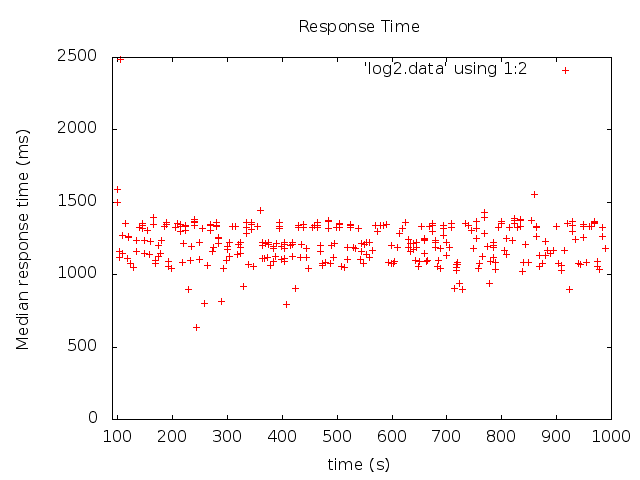
\includegraphics[scale=0.5]{src/img/out2.png}
  \caption{A benchmark evaluation with 1.0 Read-only ratio}
\label{figure:graph2}
\end{figure}

\begin{figure}[ht]
  \centering %trim=l b r t
  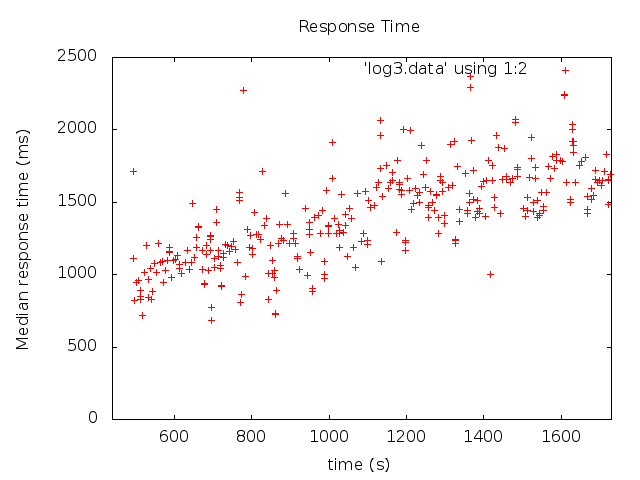
\includegraphics[scale=0.5]{src/img/out3.png}
  \caption{A benchmark evaluation with 0.4 Read-only ratio and increasing number of users}
\label{figure:graph3}
\end{figure}

\begin{figure}[ht]
  \centering %trim=l b r t
  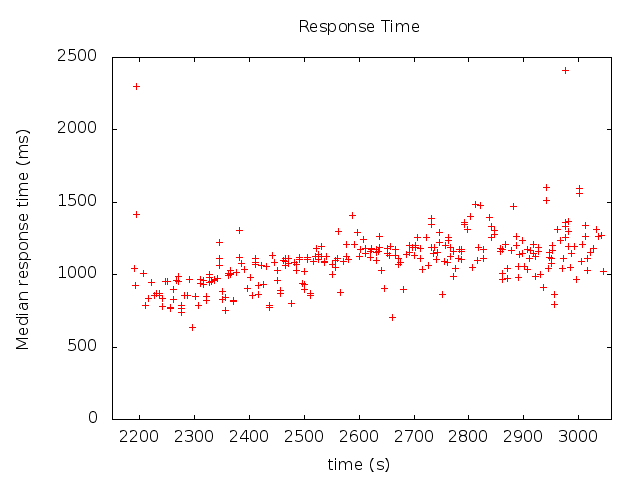
\includegraphics[scale=0.5]{src/img/out4.png}
  \caption{A benchmark evaluation with 0.4 Read-only ratio and a larger number of users}
\label{figure:graph4}
\end{figure}

\begin{figure}[ht]
  \centering %trim=l b r t
  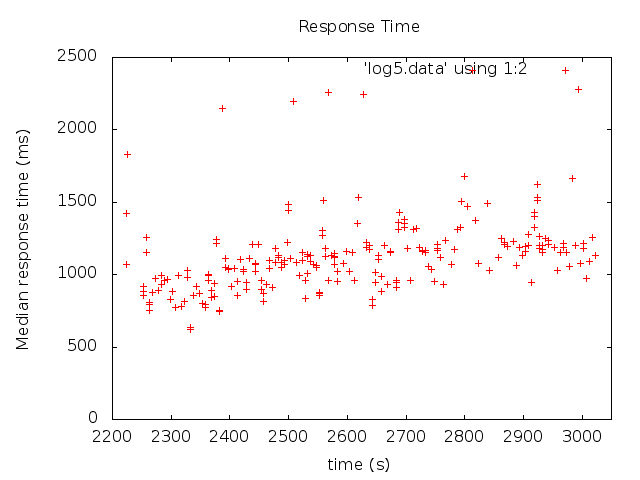
\includegraphics[scale=0.5]{src/img/out5.png}
  \caption{A benchmark evaluation with 0.4 Read-only ratio and a larger number of users}
\label{figure:graph5}
\end{figure}
